\section{Caso particolare: biforcazione con due fratture}

Come ultimo caso di studio ci siamo concentrate sulla biforcazione generata da due fratture. 

\begin{figure}[htbp]
\begin{center}
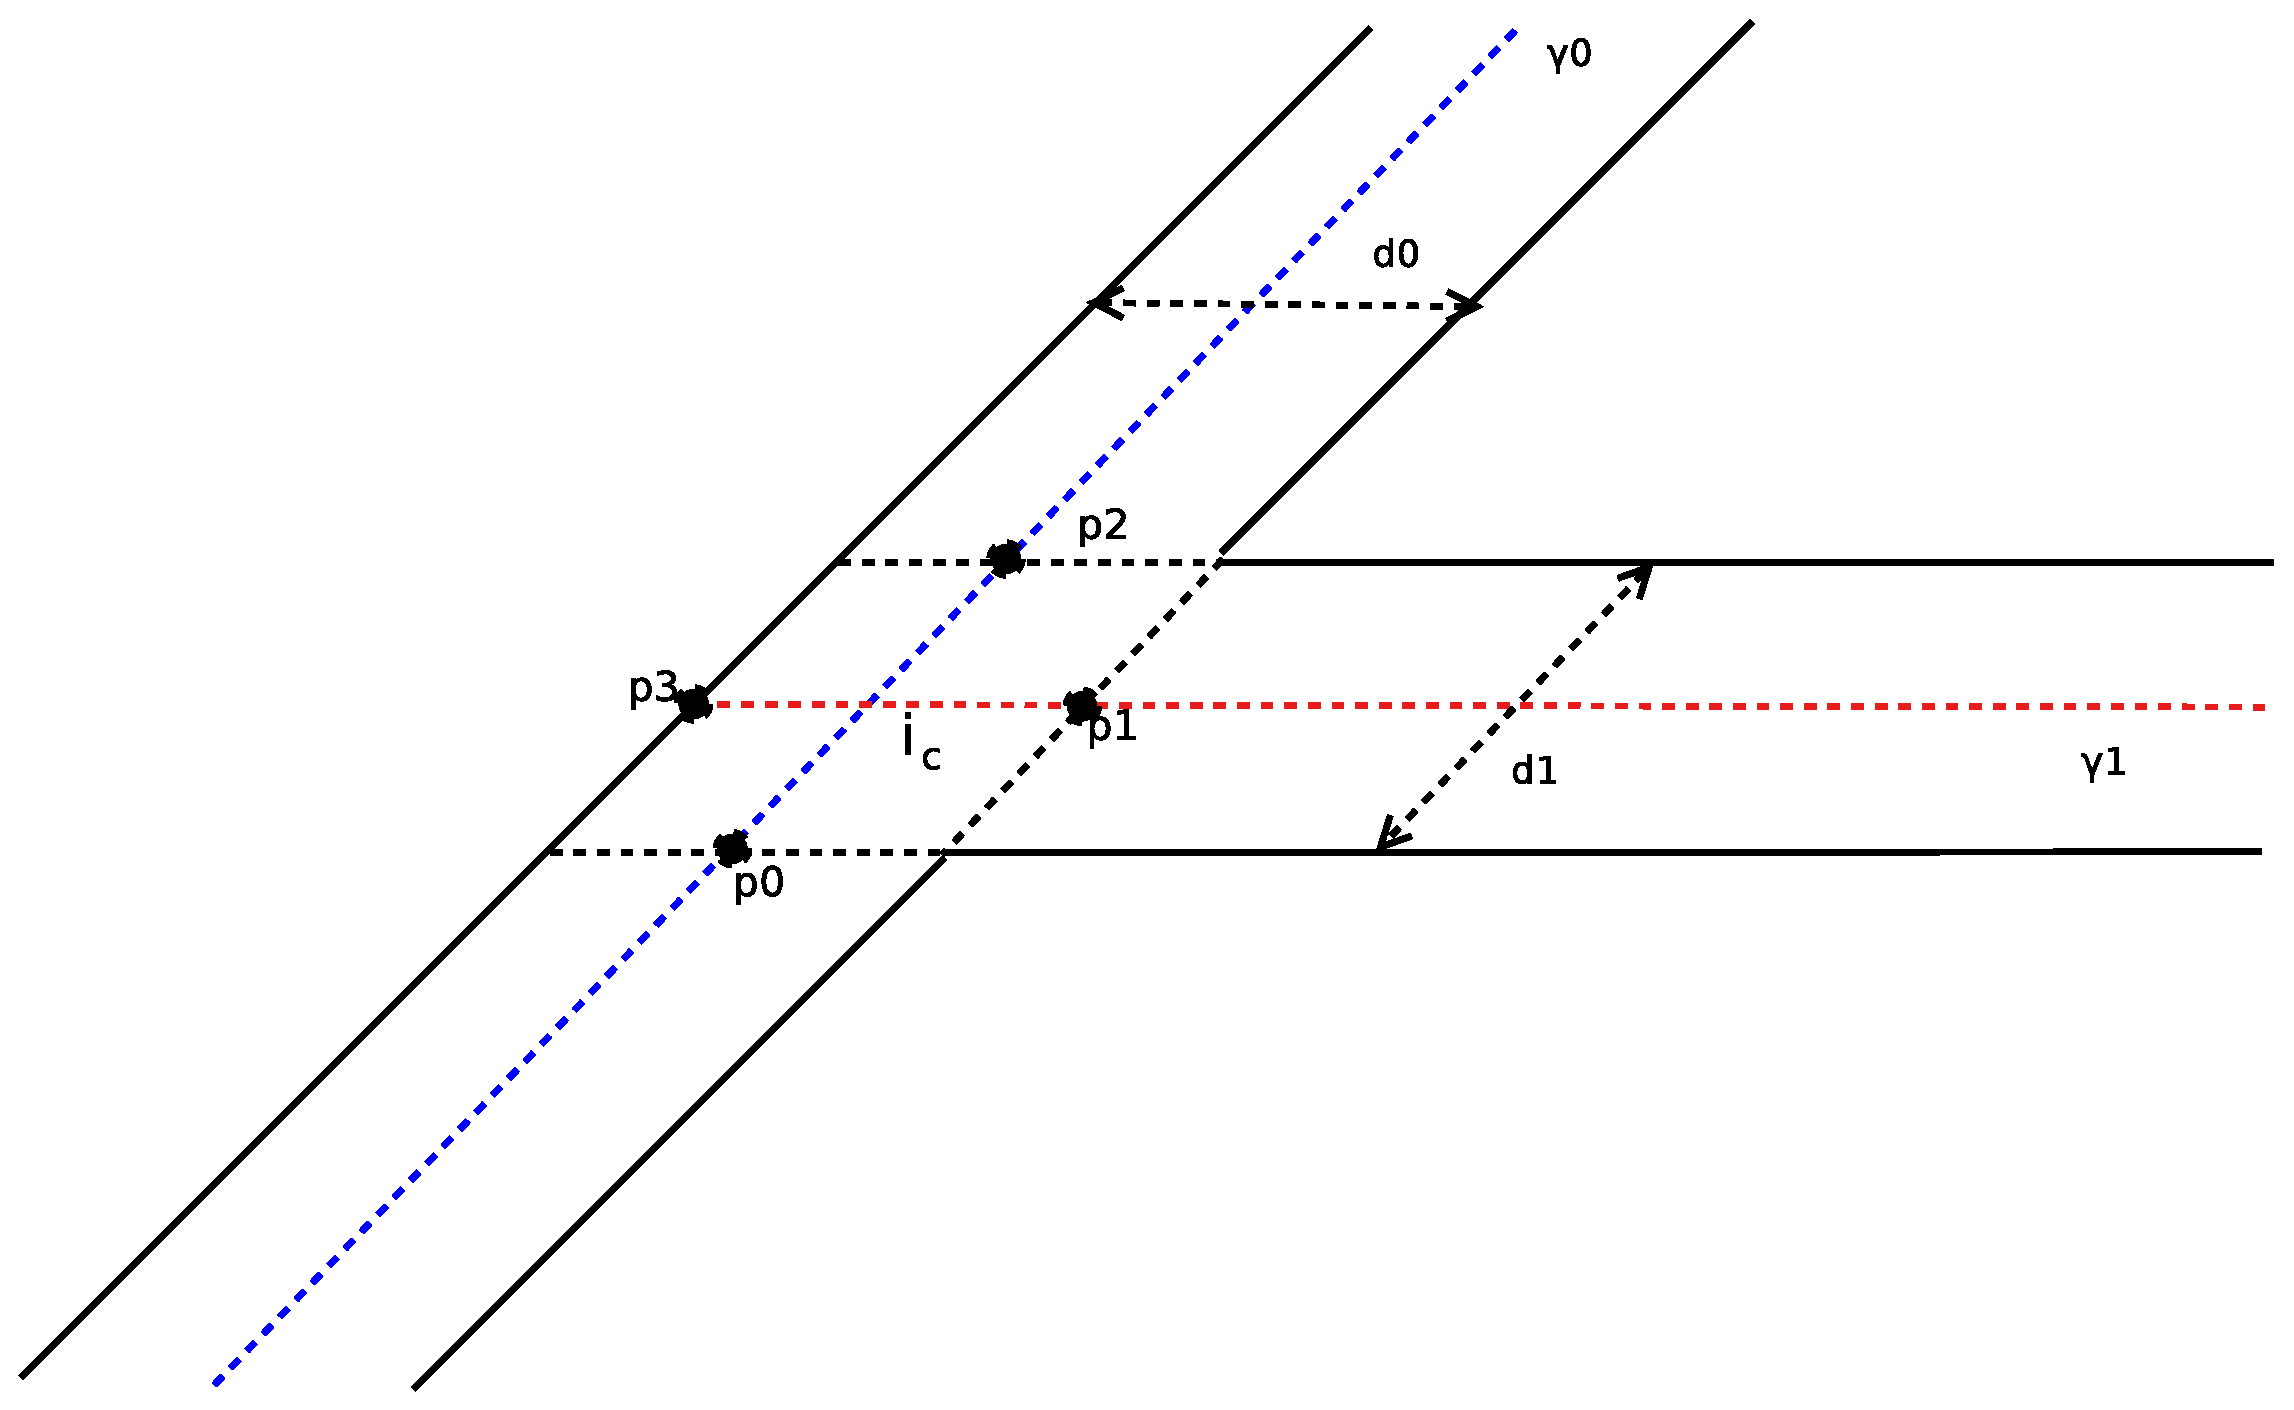
\includegraphics[width=0.8\textwidth]{img/cap6/y.eps}
\caption{Struttura di un'intersezione di tipo \textit{Bifurcation} tra due fratture.}\label{Y}
\end{center}
\end{figure}

A differenza di quanto visto fino ad ora, qui la regione d'intersezione non è più un triangolo, ma un parallelogramma. Si può generalizzare l'approssimazione fatta in \cite{Paper} con gli operatori mimetici, essendo generici e non legati al tipo di cella di integrazione su cui si lavora. \\
\noindent Il punto di intersezione $i_c$ rappresenta un punto generico per la frattura $\gamma_0$ in figura \ref{Y}, mentre per la frattura $\gamma_1$ rappresenta il primo o l'ultimo nodo. Questo punto non è detto che coincida con un nodo della mesh di $\gamma_0$ , in generale non sappiamo dove cadrà, per questo, per poter imporre le condizioni d'interfaccia in modo corretto, abbiamo introdotto per questa frattura dei gradi di libertà estesi: due per la velocità e uno per la pressione. È così possibile ottenere una miglior approssimazione del valore di velocità e pressione prima e dopo il punto di intersezione nell'elemento della mesh tagliato. \\
Esteso il codice di partenza per la costruzione del quadrilatero di intersezione, le condizioni d'interfaccia che vanno imposte hanno la stessa forma del caso delle tre fratture:

\begin{center}			
	$\left \{
		\begin{array}{l}	
	 		\textbf{u} - p_{I}T\textbf{1}_{3}+T \boldsymbol{\Pi}=0  \\ \\
     	 	\displaystyle \sum_{k=0}^3 u_{k} = p_{I} - \pi  \\
		\end{array}
	\right.$
\end{center} \label{condizioni d'interfaccia y }

\begin{figure}[htbp]
\begin{center}
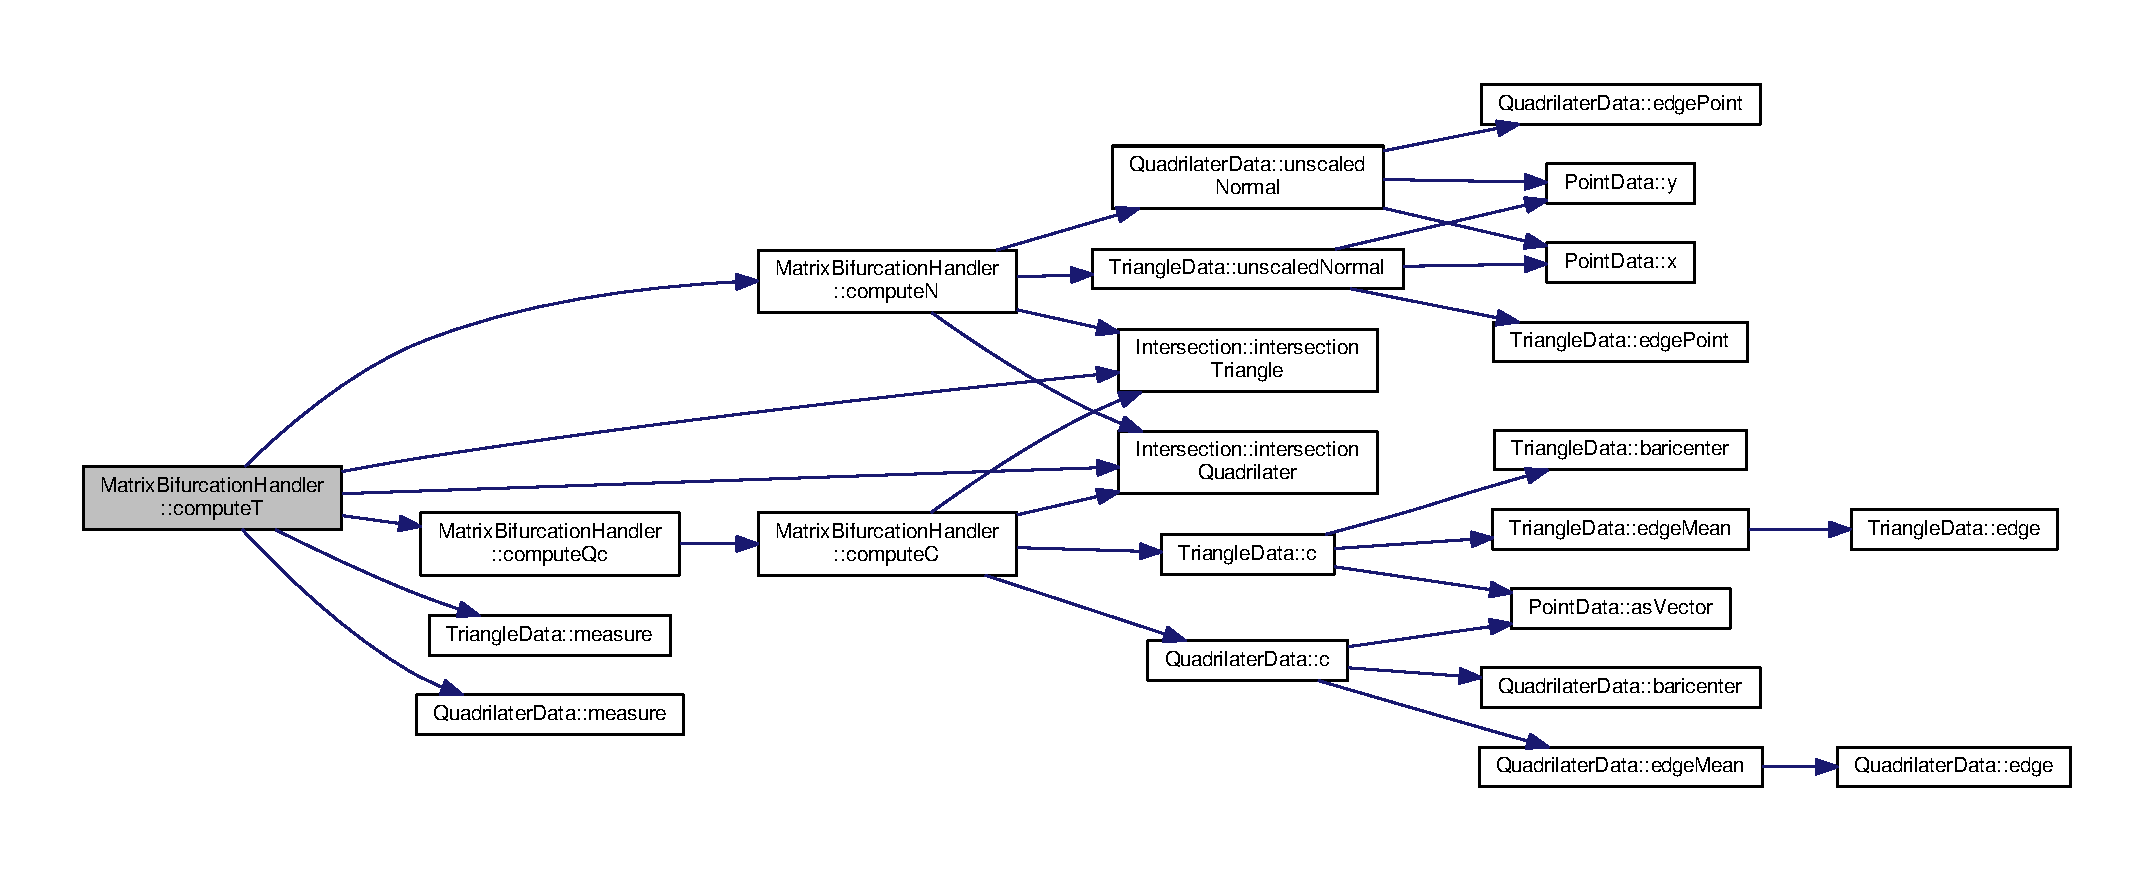
\includegraphics[width=1.2\textwidth]{img/cap6/dipendenze.pdf}
\caption{Struttura globale del codice per il calcolo generico della matrice di trasmissibilità}\label{dipendenze}
\end{center}
\end{figure}


\noindent In questo caso cambiano però le dimensioni. La matrice di trasmissibilità $T$ è ora una matrice di $\mathbb{R}^{4 \times 4}$, come diretta conseguenza della natura delle matrici $C$ e $N$. Ora infatti l'area d'intersezione è delimitata da quattro lati. Anche lo scalare $\pi$ e il vettore $\boldsymbol{\Pi}$ cambiano, e diventano:
$$\boldsymbol{\Pi} = \left[ \begin{matrix}
 			p_0\\ 
 			p_1\\
 			p_2 \\ 
		 	p_3 \\
 			\end{matrix}\right] 
$$ 
 e
$$ \pi = \frac{p_0 + p_1 + p_2 + p_3 }{4} $$

Per poter imporre le condizioni d'interfaccia, per la frattura tagliata, è necessario usare il valore della pressione e della velocità a ridosso dell'intersezione, ma questi valori sono incogniti. 
Usiamo il grado classico di pressione e il grado esteso per indicare il valore di pressione prima e dopo il punto $i_c$, indicati con $p_0$ e $p_2$ in figura \ref{Y}.  L'incognita $p_1$ rappresenta il primo o l'ultimo grado di libertà della frattura $\gamma_1$, mentre con $p_3$ indichiamo un nodo fittizio, in cui imponiamo condizione di flusso nullo.

\noindent Per quanto riguarda la velocità invece, prima dell'intersezione la poniamo pari alla media tra il valore nel grado di libertà classico prima e il valore nel grado esteso dopo il punto $i_c$. Lo stesso facciamo per il valore di velocità dopo l'intersezione, come indicato in figura \ref{xfem}. \\

\newpage
\begin{figure}[htbp]
\begin{center}
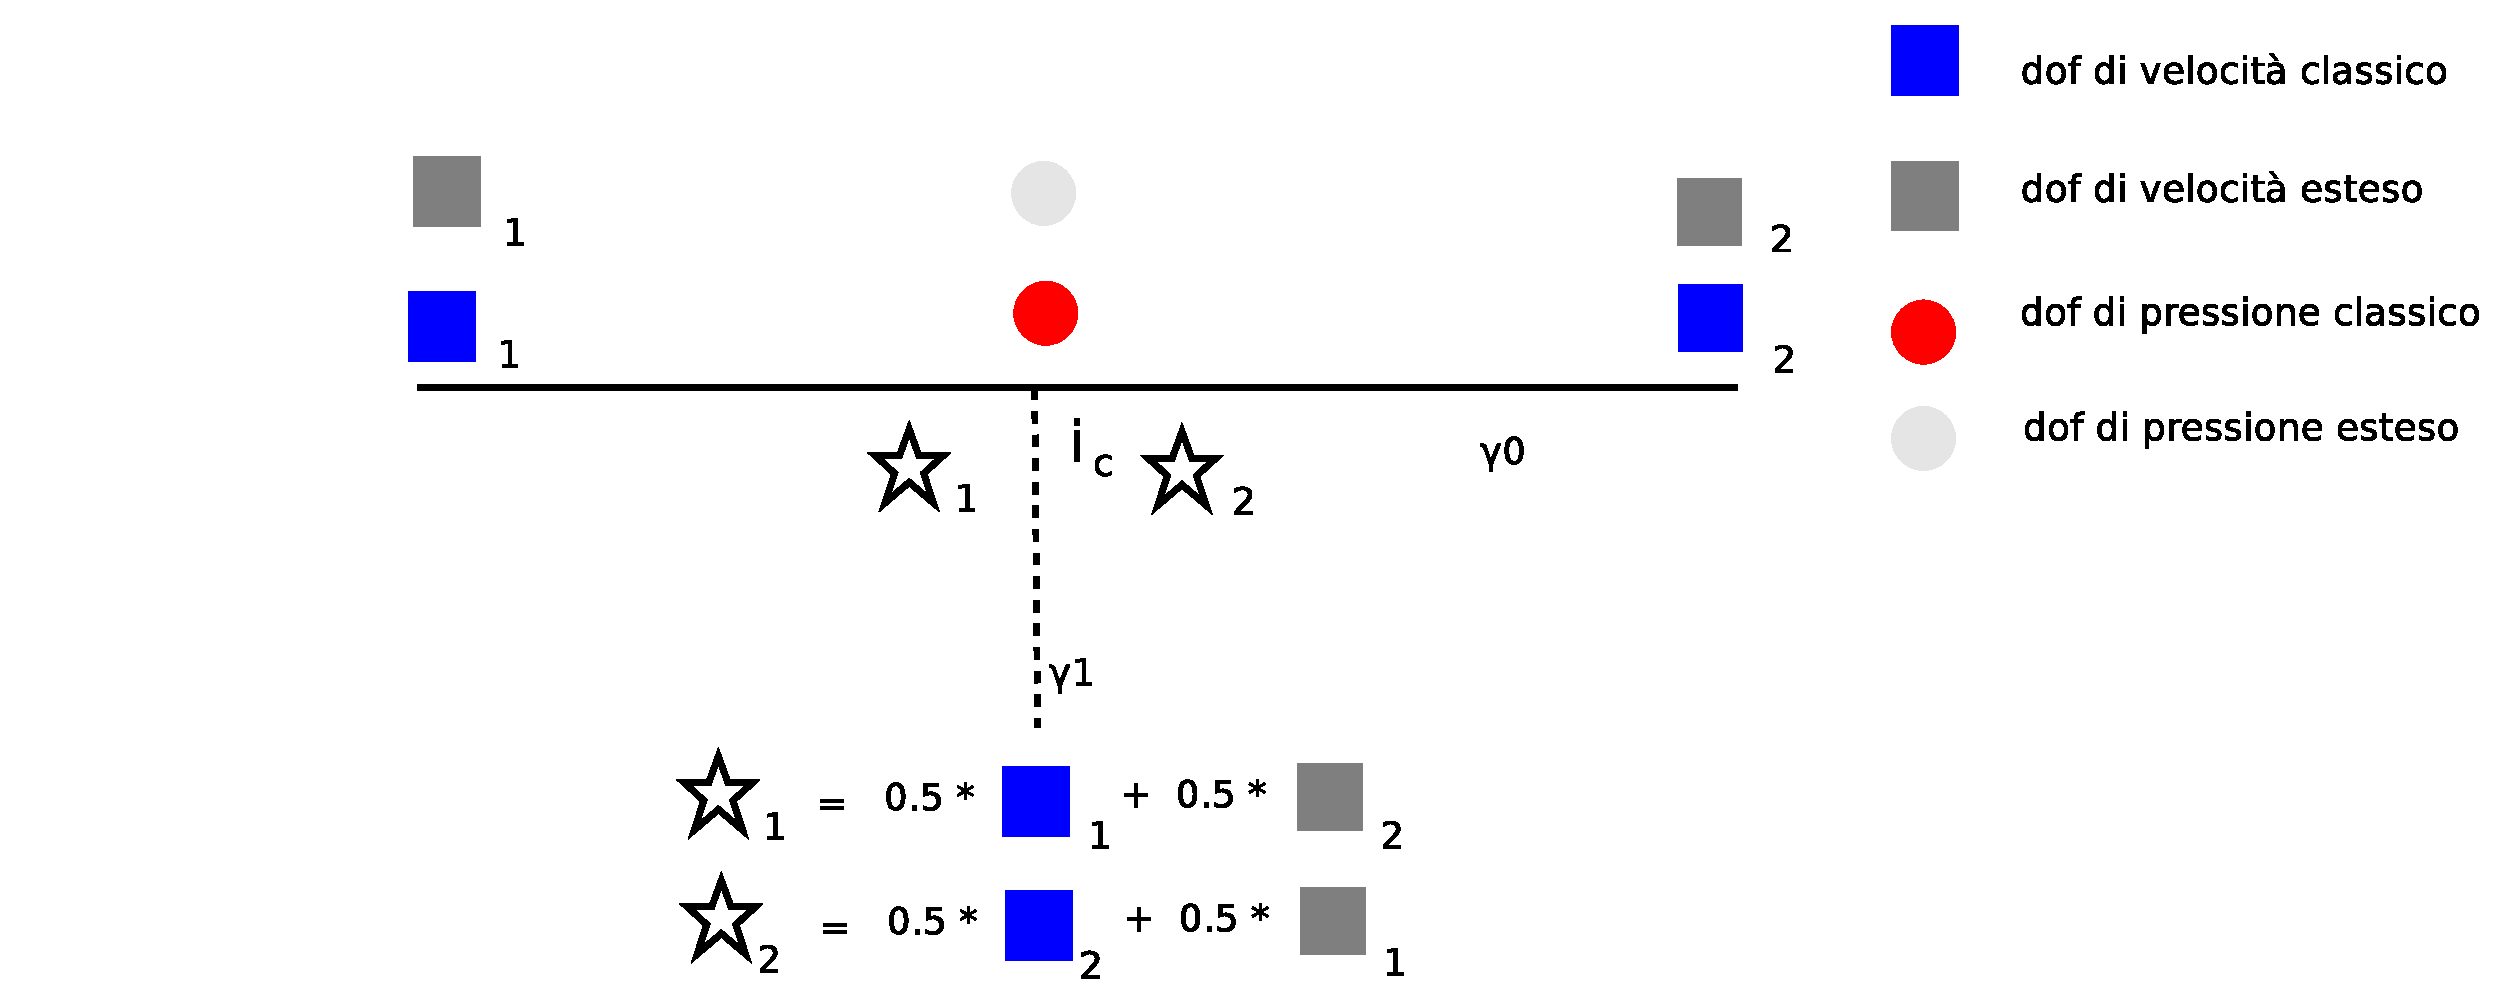
\includegraphics[width=1\textwidth]{img/cap6/xfem.eps}
\caption{Introduzione dei gradi di libertà estesi per la frattura tagliata.}\label{xfem}
\end{center}
\end{figure}

\subsection{Risultati numerici}
Ripetiamo l'analisi precedente per il caso particolare di biforcazione. Confronto valori della pressione nel DOF di intersezione per il modello 2D:\\
\begin{figure}[h!]
\centering
\includegraphics[scale=.45]{img/cap6/CP.eps}
\caption{Risultati \texttt{FreeFem++} biforcazione particolare risultati paraview }\label{CPParaview}
\end{figure}

\begin{center}
\begin{tabular}{|c|c|c|c|c|c|}
\hline
  & & \textbf{\texttt{Code}} & \multicolumn{3}{|c|}{\textbf{\texttt{FreeFem++}}} \\
\hline
\multicolumn{1}{|c|}{Frattura} & DOF & - &
\multicolumn{1}{|c|}{1E-01} & 1E-02 & 1E-03 \\
\hline
\multirow{2}{*}{0} & Base & 0.0480334 & 0.686998 & 0.303247 & 0.00685515\\
\cline{2-6}
& Esteso & 0.00295565 & 0.737573 & 0.307976 & 0.00665541\\
\hline
 1 & Base & 0.0146871 & 0.637801 & 0.298043 & 0.00673082\\
\hline
\end{tabular}
\end{center}

\begin{center}
\begin{tabular}{|c|c|c|c|}
\hline
\multicolumn{4}{|c|}{Pressione media} \\
\hline
\textbf{\texttt{Code}} & \multicolumn{3}{|c|}{\textbf{\texttt{FreeFem++}}} \\
\hline
- & \multicolumn{1}{|c|}{1E-01} & 1E-02 & 1E-03 \\
\hline
0.02189205 & 0.679653 & 0.301661 & 0.00672457 \\
\hline
\end{tabular}
\end{center}

\begin{figure}[h!]
\centering
\includegraphics[scale=.07]{img/cap6/BifuY.eps}
\caption{Risultati \texttt{FreeFem++} biforcazione con due fratture - spessore ordine 1E-02 }\label{Biforcazione2Frat1E-02}
\end{figure}

\begin{center}
\begin{tabular}{|c|c|c|}
\hline
  \multicolumn{3}{|c|}{\textbf{\texttt{Errore}}} \\ 
\hline
\multicolumn{1}{|c|}{1E-01} & 1E-02 & 1E-03 \\
\hline
0.65776095 & 0.27976895 & 0.01516748 \\
\hline
\end{tabular}
\end{center}

\subsection{Conclusioni}
Dal confronto dei risultati ottenuti con il nostro codice e con i codici \texttt{FreeFem++} possiamo concludere che effettivamente il modello ridotto da noi usato rappresenta una buona approssimazione del fenomeno. L'approssimazione è tanto migliore quanto più le fratture hanno uno spessore piccolo, come avevamo già previsto. Infatti più sono grandi e più informazioni trascuriamo usando un modello 1d. \\
\noindent Si potrebbe generalizzare ulteriormente il codice, usando sempre gli operatori mimetici, al caso in cui vi sia un numero generico di fratture che si intersecano in un punto. 
